\documentclass[modern]{aastex62}

\usepackage{graphicx}
\usepackage{xcolor}
\usepackage{xspace}
\usepackage[sort&compress]{natbib}
\usepackage[hang,flushmargin]{footmisc}


% style tweaks
\newcommand{\acronym}[1]{{\small{#1}}}
\newcommand{\project}[1]{\textsl{#1}}
\newcommand{\code}[1]{{\texttt{#1}}}
\newcommand{\todo}[1]{\textcolor{red}{#1}}

% the following is stolen from Adrian Price-Whelan (github.com/adrn/latex-init):
\usepackage{hyperref}
\definecolor{niceblue}{rgb}{0.0, 0.4, 0.65}
\definecolor{linkcolor}{rgb}{0.02,0.35,0.55}
\definecolor{citecolor}{rgb}{0.4,0.4,0.4}
\hypersetup{colorlinks=true,linkcolor=linkcolor,citecolor=citecolor,
            filecolor=linkcolor,urlcolor=linkcolor}
\hypersetup{pageanchor=false}

% astronomy
\newcommand{\teff}{\ensuremath{T_{\rm eff}}}
\newcommand{\logg}{\ensuremath{\log g}}
\newcommand{\feh}{\ensuremath{\mathrm{[Fe/H]}}}
\newcommand{\vt}{\ensuremath{v_t}}
\newcommand{\mh}{\ensuremath{\mathrm{[M/H]}}}
\newcommand{\xh}{\ensuremath{\mathrm{[X/H]}}}
\newcommand{\I}{\textsc{I}}
\newcommand{\II}{\textsc{II}}
\newcommand{\vsini}{\ensuremath{v \sin{i}}}
\newcommand{\gcm}{\ensuremath{\mathrm{g}~\mathrm{cm}^{-3}}}
\newcommand{\kms}{\ensuremath{\mathrm{km}~\mathrm{s}^{-1}}}
\newcommand{\masyr}{\ensuremath{\mathrm{mas}~\mathrm{yr}^{-1}}}
\newcommand{\msun}{\ensuremath{\mathrm{M}_\odot}}
\newcommand{\ang}{\text{\normalfont\AA}}


\newcommand{\TF}{\code{TensorFlow}\xspace}
\newcommand{\python}{\code{python}\xspace}
\newcommand{\HARPS}{\project{\acronym{HARPS}}\xspace}
\newcommand{\HIRES}{\project{\acronym{HIRES}}\xspace}
\newcommand{\RV}{\acronym{RV}\xspace}
\newcommand{\RVs}{\acronym{RV}s\xspace}


% stolen from Ben Pope:
\newcommand{\kepler}{\emph{Kepler}\xspace}
\newcommand{\hipparcos}{\emph{Hipparcos}\xspace}
\newcommand{\gaia}{\emph{Gaia}\xspace}
\newcommand{\ktwo}{\emph{K2}\xspace}
\newcommand{\TESS}{\emph{\acronym{TESS}}\xspace}

% misc shortcuts
\newcommand{\flatiron}{Flatiron Institute, Simons Foundation, 162 Fifth Ave, New York, NY 10010, USA}
\newcommand{\chicago}{Department of Astronomy and Astrophysics, University of
Chicago, 5640 S. Ellis Ave, Chicago, IL 60637, USA}
\newcommand{\USP}{Universidade de Sao Paulo}
\newcommand{\MIT}{MIT}

\graphicspath{ {./figures/} }
\newcommand{\hoststar}{\acronym{HIP}\ 96160\xspace}
\newcommand{\plname}{\acronym{HIP}\ 96160b\xspace}
\newcommand{\plmass}{$13.1 \pm 5.0\ \textrm{M}_{E}$\xspace}
\newcommand{\plradius}{$3.41 \pm 0.01\ \textrm{R}_{E}$\xspace}
\newcommand{\stmass}{$1.0 \pm x\ \textrm{M}_{\odot}$\xspace}
\newcommand{\stradius}{$1.0 \pm x\ \textrm{R}_{\odot}$\xspace}

\shorttitle{Warm Sub-Neptune Transiting a Solar Twin}
\shortauthors{Bedell et al.}

\setlength{\parindent}{1.4em} % trust in Hogg
\begin{document}\sloppy\sloppypar\raggedbottom\frenchspacing % trust in Hogg

\graphicspath{ {figures/} }
\DeclareGraphicsExtensions{.pdf,.eps,.png}

\title{A Warm Sub-Neptune Transiting a Solar Twin in TESS}

\author[0000-0001-9907-7742]{Megan Bedell}
\affiliation{\flatiron}

\author{Dan Foreman-Mackey}
\affiliation{\flatiron}

\author{Chelsea Huang}
\affiliation{\MIT}

\author{Jennifer Burt}
\affiliation{\MIT}

\author{Jorge Melendez}
\affiliation{\USP}

\author{Jhon Yana Galarza}
\affiliation{\USP}

\author{Lorenzo Spina}
\affiliation{Monash}

%\author{Jacob L. Bean}
%\affiliation{\chicago}


\author{\todo{other STPS folks}}



\correspondingauthor{Megan Bedell}
\email{mbedell@flatironinstitute.org}


\begin{abstract}\noindent
We present the discovery of \plname, a sub-Neptune planet transiting a nearby solar twin star. 
The host star has been observed extensively as part of a radial velocity (\RV) campaign targeting solar twins with \HARPS. 
From these data, we find a planetary minimum mass of \plmass. 
We also measure a radius of \plradius from \TESS photometry. 
Taken together, the resulting planetary bulk density of \pldensity implies that an extended atmosphere is present, making this system an excellent candidate for transmission spectroscopic follow-up. 
The extreme similarity between \hoststar and the Sun means that both the absolute planetary mass and radius and the bulk composition of the \hoststar system can be measured to unusually high precision. 
\todo{We use the composition of the host star to place constraints on the planet's potential properties and show that it is likely to be... ??}

% Precise characterization of exoplanet host stars is critical to our understanding of their properties. 
% However, stellar spectroscopic characterization can be plagued with 
\end{abstract}


\section{Introduction}
\label{s:intro}

The Transiting Exoplanet Survey Satellite (\TESS) has detected over one thousand candidate exoplanets to date. 
The majority of these newly discovered planets orbit bright, nearby stars, making them perfectly suited for follow-up observations, including mass measurements and atmospheric spectroscopy. 
Unlike most \kepler systems, then, observational signal-to-noise is not always the dominant term in the error budget for the planet masses and other properties measured by ground-based follow-up campaigns.

(importance of solar twins)

In this work, we present the first planet detected by \TESS to orbit a true solar twin star. 
\object[HIP96160]{\hoststar} is a \stmass, \stradius G2V star with a spectrum nearly identical to that of the Sun. 
Previous studies have derived stellar properties and photospheric abundances for this \hoststar that are accurate to the $1-2 \%$ level.

%All 

%\hoststar has been studied extensively through a dedicated \RV planet search and spectroscopic abundance survey targeting solar twin stars. ...

\section{Data}
\label{s:data}

\subsection{Photometry}

\hoststar was observed at 2-minute cadence as part of \TESS Sector 13. 


\subsection{Spectra}

(about \HARPS\ \RVs)

(about co-added spectrum - SNR etc)

\subsection{Gaia}

(cross-match. nearby stars?)

\section{Analysis \& Results}
\label{s:analysis}

\subsection{Stellar Characterization}
\label{s:analysis:star}


(cite spectroscopic properties + abundances from previous work, plus Gaia DR2)
(isochrones fit - we use this mass \& radius going forward)

(attempts at seismology \& rotation period)

\subsection{Photometric Analysis}
\label{s:analysis:photometry}

(transits visible by eye, TOI flagging)

(centroid analysis?)

(GP model \& discussion of physical meaning - is this rotation period?)

(results of planet-only fit)

\begin{figure}
    \centering
    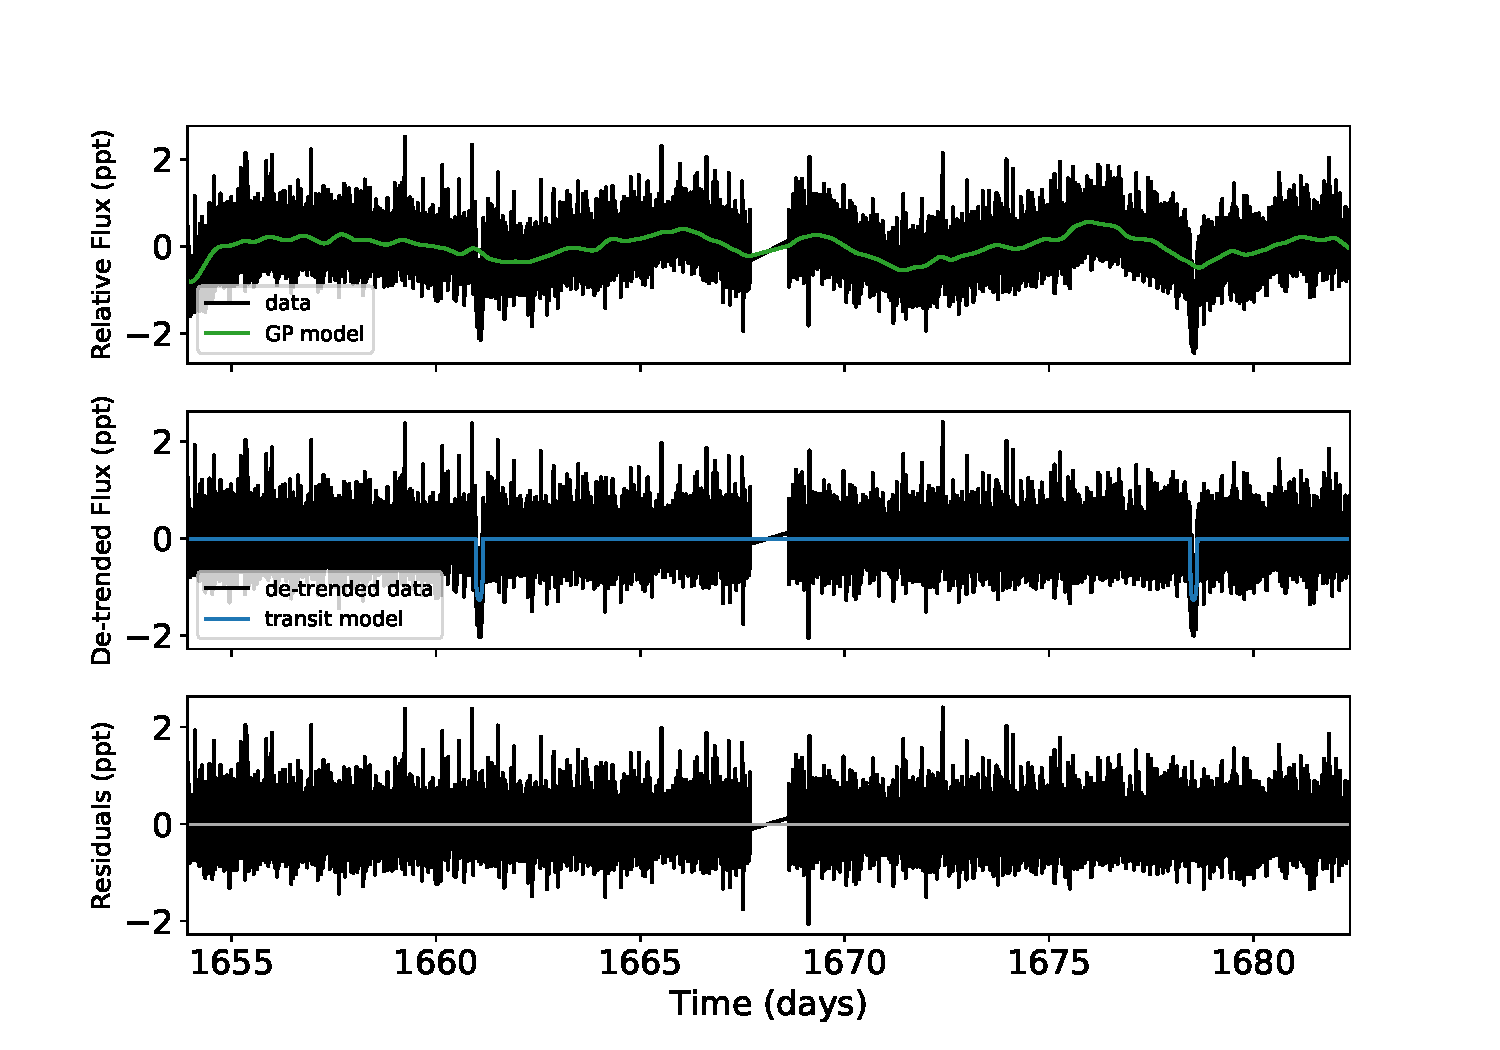
\includegraphics[width=\textwidth]{lightcurve.pdf}
    \caption{Photometric lightcurve of \hoststar as observed by \TESS in Sector 13. The \TESS data were fit with a Gaussian Process model (top panel) as a means of detrending. A transit model was then fit (middle panel), leaving a featureless white-noise lightcurve in the residuals (bottom panel).}
    \label{fig:lightcurve}
\end{figure}

\subsection{\RV Analysis}
\label{s:analysis:rvs}

(\HARPS\ upgrade offset)

(what do logRHK, BIS, FWHM correlations look like \& their periodograms after removing this offset (\& maybe low-pass filtering??))

\begin{figure}
    \centering
    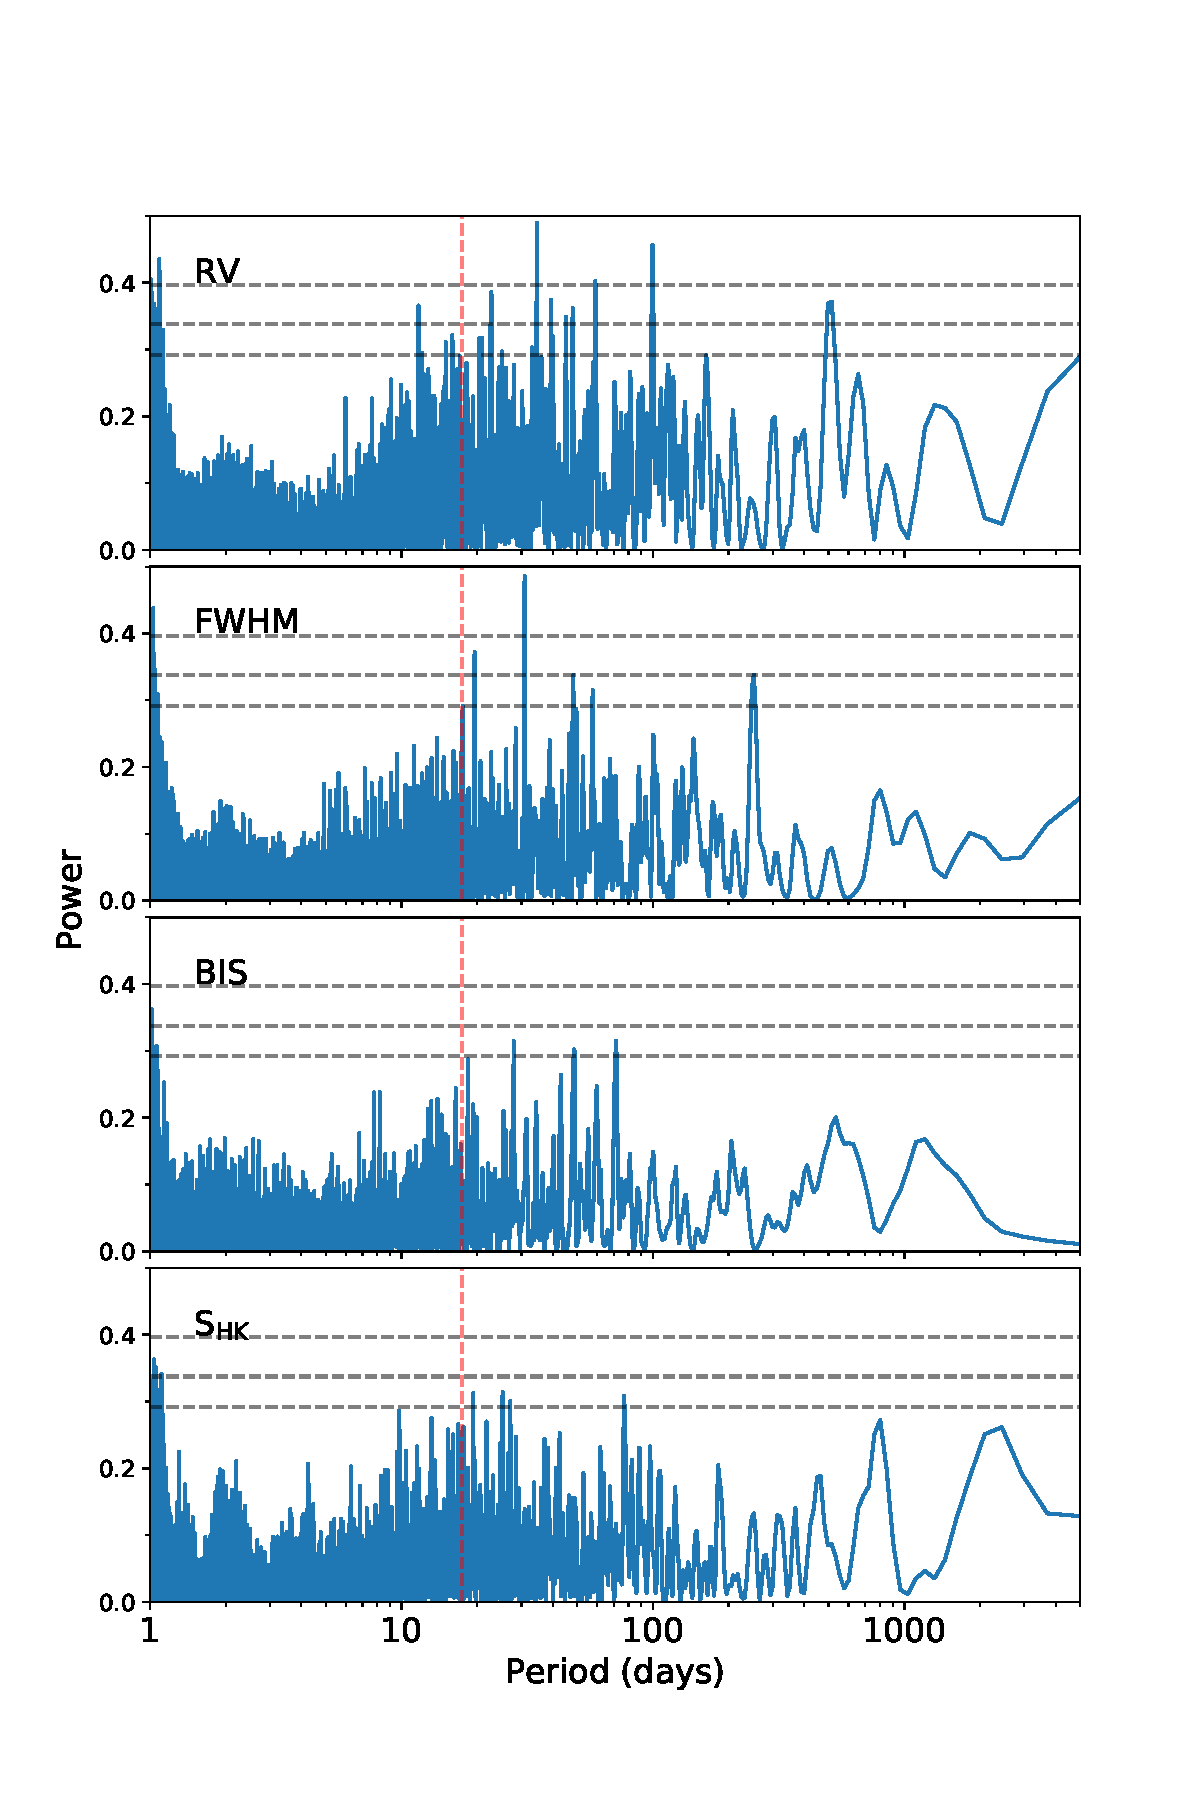
\includegraphics[width=\textwidth]{periodograms.pdf}
    \caption{Lomb-Scargle periodograms of the \HARPS \RV, BIS, FWHM, and \shk timeseries measurements. Horizontal lines indicate the 5\%, 1\%, and 0.1\% false alarm probability levels. Vertical red lines mark the period of the \TESS-detected planet. The \RV, BIS, and FWHM measurements used here have been corrected for the \HARPS upgrade offset.}
    \label{fig:periodograms}
\end{figure}

(periodogram analysis of RVs (maybe after subtracting off activity trends))

\begin{figure}
    \centering
    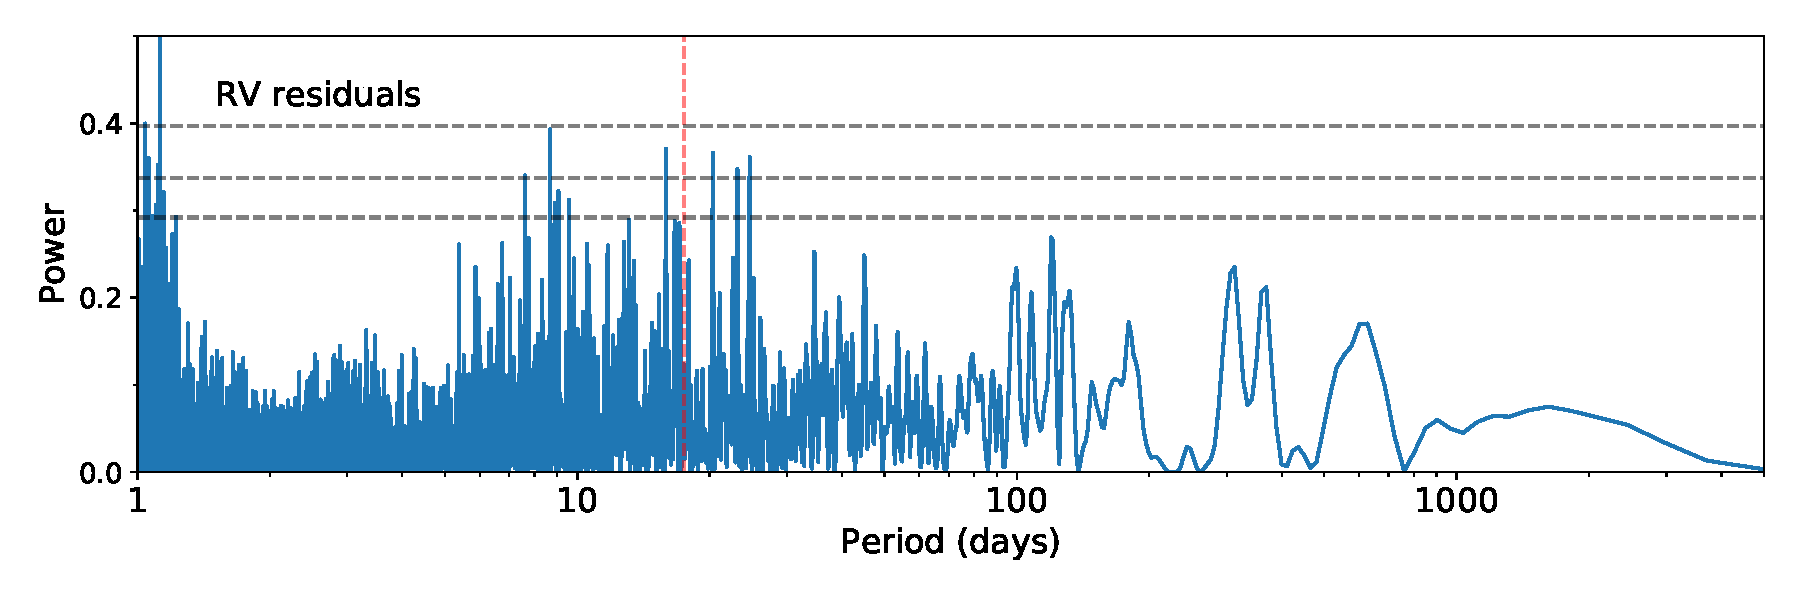
\includegraphics[width=\textwidth]{periodogram_resids1.pdf}
    \caption{Lomb-Scargle periodogram of the \RV residuals after subtracting the best-fit no-planet model consisting of a quadratic trend, a linear correlation with FWHM, and an instrumental offset after the time of the \HARPS upgrade.}
    \label{fig:periodogram_resids1}
\end{figure}

(adding a planet to the model)

(evidence for additional periods?)

\subsection{Joint Analysis}
\label{s:analysis:joint}


\section{Discussion}
\label{s:discussion}


(Low probability of background contaminants - discuss Gaia, spectra)

(reliability of the RV fit - potential for more planets? activity?)

(M-R diagram)

(prospects for further compositional analysis)

(prospects for atmospheric characterization)

\section{Conclusion}
\label{s:conclusion}


\acknowledgements
We thank ...

\software{
    \code{Astropy} \citep{astropy},
    \code{exoplanet} \citep{exoplanet},
    \code{IPython} \citep{ipython},
    \code{matplotlib} \citep{matplotlib},
    \code{numpy} \citep{numpy},
    \code{scipy} (\url{https://www.scipy.org/}),
}

\facility{TESS, HARPS}

\bibliographystyle{aasjournal}
\bibliography{ms}

\end{document}